\documentclass[11pt,a4paper]{article}

\usepackage{fontspec}
\usepackage[polish]{babel}
\setmainfont{[lmroman10-regular.otf]}[
    BoldFont = {[lmroman10-bold.otf]},
    ItalicFont = {[lmroman10-italic.otf]},
    BoldItalicFont = {[lmroman10-bolditalic.otf]}
]
\setsansfont{[lmsans10-regular.otf]}[
    BoldFont = {[lmsans10-bold.otf]}
]
\setmonofont{[lmmono10-regular.otf]}
\usepackage{graphicx}
\usepackage[table]{xcolor}
\usepackage{tabularx}
\usepackage{array}
\usepackage{geometry}
\usepackage{hyperref}
\usepackage{enumitem}
\usepackage{fancyhdr}
\usepackage{listings}
\usepackage{tcolorbox}
\usepackage{float}
\usepackage{needspace}
\tcbuselibrary{breakable}

\geometry{left=2cm,right=2cm,top=1.7cm,bottom=1.8cm}
\setlength{\parindent}{0pt}
\setlength{\parskip}{5pt}

\definecolor{PSblue}{HTML}{1F5B99}
\definecolor{PSlight}{HTML}{EAF2F8}
\definecolor{PSgray}{HTML}{5F6B76}

\hypersetup{colorlinks=true,urlcolor=PSblue,linkcolor=PSblue}
\pagestyle{fancy}
\fancyhf{}
\fancyfoot[C]{\small\color{PSgray}Aplikacje webowe i sieciowe -- Politechnika Śląska}
\renewcommand{\headrulewidth}{0pt}

\newcommand{\pole}[1]{\textit{#1}}
\newcommand{\zadanie}{Laboratorium 1 -- Szkielet ASP.NET Core Web API w architekturze warstwowej (CarsWebApplication), rozszerzony o pełny zestaw operacji CRUD}
\newcommand{\punkty}{..............}
\newcommand{\skladsekcji}{Piotr Lasoń (grupa 3)}

\begin{document}

\begin{minipage}[c]{0.25\textwidth}
    \IfFileExists{LogoPSl.jpg}{\includegraphics[width=3.0cm]{LogoPSl.jpg}}{\fbox{\parbox[c][2.7cm][c]{3cm}{\centering Logo PŚ}}}
\end{minipage}%
\begin{minipage}[c]{0.75\textwidth}
    \raggedleft
    {\Large\bfseries\color{PSblue} APLIKACJE WEBOWE I SIECIOWE}\\[2mm]
    {\small\color{PSgray}Formatka dokumentacji zadania}
\end{minipage}

\vspace{2mm}
{\color{PSblue}\rule{\textwidth}{1.2pt}}
\vspace{4mm}

\begin{center}
{\LARGE\bfseries\color{PSblue} Dokumentacja wykonania zadania}\\[1mm]
{\small\color{PSgray}Szablon do zadań punktowanych realizowanych podczas laboratoriów}
\end{center}

\vspace{3mm}

\renewcommand{\arraystretch}{1.45}
\begin{tabularx}{\textwidth}{>{\bfseries\color{PSblue}\columncolor{PSlight}}p{4.6cm} X}
Przedmiot & Aplikacje webowe i sieciowe \\
Kierunek studiów & Informatyka \\
Forma i poziom studiów & studia stacjonarne I stopnia (inżynierskie), semestr 5 \\
Prowadzący & dr inż. Rafał Brociek \\
Skład sekcji / Imię i nazwisko & \skladsekcji \\
Zadanie & \zadanie \\
Liczba punktów & \punkty \\
\end{tabularx}

\section*{\color{PSblue}1. Zakres wykonanego zadania}
{\small\color{PSgray}\textit{Krótko opisz, co zostało wykonane w ramach zadania. Wskaż najważniejsze elementy rozwiązania i uzyskany rezultat.}}

\begin{tcolorbox}[breakable,colback=gray!2,colframe=gray!25,boxrule=0.5pt,arc=1mm]
Zrealizowano szkielet backendu \texttt{CarsWebApplication} w architekturze warstwowej, zgodnie z instrukcją do Laboratorium~1. Solucja składa się z czterech projektów: \texttt{Cars.Domain} (model \texttt{Car} oraz wyliczenia \texttt{FuelType}, \texttt{BodyType}, bez zależności od innych warstw), \texttt{Cars.Application} (projekt-placeholder pod przyszłą logikę biznesową, zależny od \texttt{Cars.Domain}), \texttt{Cars.Infrastructure} (kontekst bazy danych \texttt{DataContext} oparty na EF~Core + SQLite, migracja \texttt{InitialCreate} oraz dane startowe \texttt{Seed}) i \texttt{Cars.API} (projekt startowy, kontrolery REST, konfiguracja CORS i rejestracja usług w \texttt{Program.cs}).

Baza danych SQLite (\texttt{cars.db}) jest tworzona i migrowana automatycznie przy starcie aplikacji, a następnie wypełniana trzema przykładowymi samochodami, o ile tabela jest pusta.

W stosunku do zakresu podstawowego instrukcji (same odczyty), kontroler \texttt{CarsController} został rozszerzony -- zgodnie z sekcją ,,Co dalej?'' instrukcji -- o pełny zestaw operacji CRUD: \texttt{GET~/api/cars}, \texttt{GET~/api/cars/\{id\}}, \texttt{POST~/api/cars}, \texttt{PUT~/api/cars/\{id\}} oraz \texttt{DELETE~/api/cars/\{id\}}. Wszystkie endpointy zostały ręcznie przetestowane (curl oraz podgląd w przeglądarce) i działają zgodnie z oczekiwaniami, zwracając poprawne kody odpowiedzi (200, 201, 204, 404).

Dodatkowo, poza samym dokumentem OpenAPI (\texttt{/openapi/v1.json}), w projekcie \texttt{Cars.API} skonfigurowano pakiet \texttt{Swashbuckle.AspNetCore}, dzięki czemu pod adresem \texttt{/swagger} dostępny jest interaktywny Swagger~UI pozwalający przeglądać i testować wszystkie endpointy bezpośrednio z przeglądarki (zrzuty ekranu poniżej).
\end{tcolorbox}

\section*{\color{PSblue}2. Dokumentacja rozwiązania}
{\small\color{PSgray}\textit{W razie potrzeby zamieść kluczowe fragmenty kodu, krótkie objaśnienia, zrzuty ekranu lub inne elementy potwierdzające wykonanie zadania. Nie wklejaj całego kodu źródłowego.}}

\subsection*{Architektura i zależności projektów}
\begin{itemize}[nosep]
    \item \texttt{Cars.Domain} -- nie zależy od żadnego projektu,
    \item \texttt{Cars.Application} -- zależy od \texttt{Cars.Domain},
    \item \texttt{Cars.Infrastructure} -- zależy od \texttt{Cars.Domain},
    \item \texttt{Cars.API} -- zależy od \texttt{Cars.Application} oraz \texttt{Cars.Infrastructure}.
\end{itemize}

\subsection*{Model danych (\texttt{Cars.Domain/Car.cs})}
\begin{lstlisting}[basicstyle=\footnotesize\ttfamily,breaklines=true,frame=single]
public class Car
{
    public Guid Id { get; set; }
    public string Brand { get; set; } = string.Empty;
    public string Model { get; set; } = string.Empty;
    public int DoorsNumber { get; set; }
    public int LuggageCapacity { get; set; }
    public int EngineCapacity { get; set; }
    public FuelType FuelType { get; set; }
    public DateTime ProductionDate { get; set; }
    public double AverageFuelConsumption { get; set; }
    public BodyType BodyType { get; set; }
}
\end{lstlisting}

\subsection*{Kontroler \texttt{CarsController} -- przykładowe endpointy}
Kontroler dziedziczy po \texttt{BaseApiController} (\texttt{[Route("api/[controller]")]}) i korzysta bezpośrednio z \texttt{DataContext} (zgodnie z celowym uproszczeniem przyjętym na tym etapie zajęć). Poniżej fragment ilustrujący odczyt listy oraz dodawanie rekordu -- pozostałe operacje (\texttt{GetCar}, \texttt{UpdateCar}, \texttt{DeleteCar}) mają analogiczną budowę.

\begin{lstlisting}[basicstyle=\footnotesize\ttfamily,breaklines=true,frame=single]
[HttpGet]
public async Task<ActionResult<List<Car>>> GetCars()
{
    return await _context.Cars.AsNoTracking().ToListAsync();
}

[HttpPost]
public async Task<ActionResult<Car>> CreateCar(Car car)
{
    car.Id = Guid.NewGuid();
    _context.Cars.Add(car);
    await _context.SaveChangesAsync();
    return CreatedAtAction(nameof(GetCar), new { id = car.Id }, car);
}
\end{lstlisting}

\subsection*{Zaimplementowane endpointy}
\renewcommand{\arraystretch}{1.3}
\begin{tabularx}{\textwidth}{>{\bfseries\color{PSblue}\columncolor{PSlight}}p{3.4cm} p{4.3cm} X}
Endpoint & Opis & Kody odpowiedzi \\
\texttt{GET /api/cars} & lista wszystkich samochodów & 200 OK \\
\texttt{GET /api/cars/\{id\}} & pobranie jednego samochodu & 200 OK / 404 Not Found \\
\texttt{POST /api/cars} & dodanie nowego samochodu & 201 Created \\
\texttt{PUT /api/cars/\{id\}} & aktualizacja istniejącego samochodu & 204 No Content / 400 / 404 \\
\texttt{DELETE /api/cars/\{id\}} & usunięcie samochodu & 204 No Content / 404 Not Found \\
\end{tabularx}

\Needspace{11cm}
\subsection*{Zrzuty ekranu -- Swagger UI}

\begin{figure}[H]
    \centering
    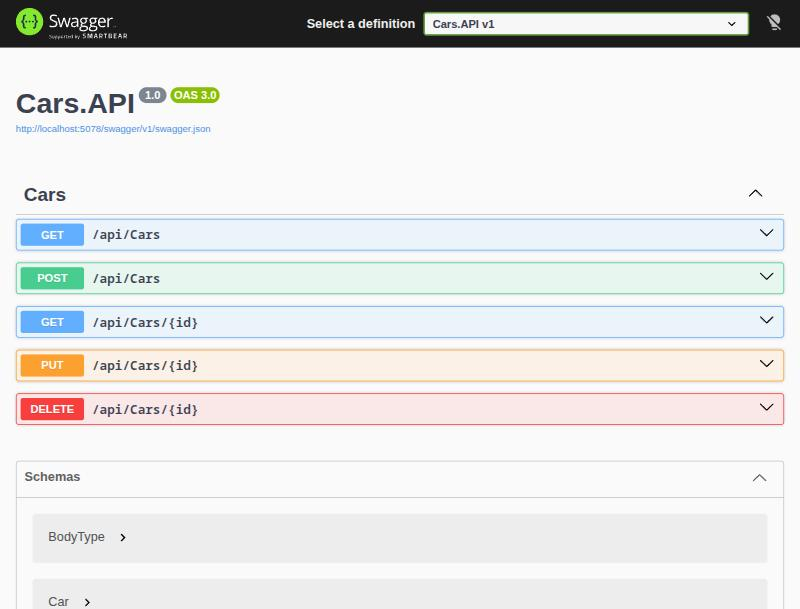
\includegraphics[width=0.66\textwidth]{img/swagger-overview.jpg}
    \caption{Swagger UI (\texttt{/swagger}) -- widok wszystkich pięciu endpointów kontrolera \texttt{CarsController}: \texttt{GET}, \texttt{POST}, \texttt{GET/\{id\}}, \texttt{PUT/\{id\}}, \texttt{DELETE/\{id\}}.}
\end{figure}

\Needspace{11cm}
\begin{figure}[H]
    \centering
    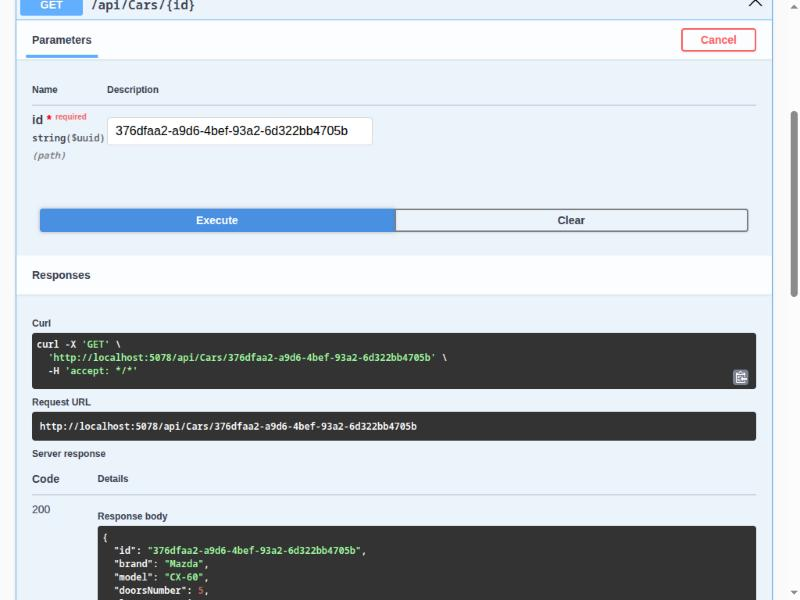
\includegraphics[width=0.66\textwidth]{img/swagger-get-by-id.jpg}
    \caption{Swagger UI -- wywołanie \texttt{GET /api/Cars/\{id\}} przez ,,Try it out'' wraz z wygenerowanym poleceniem curl i odpowiedzią 200 z danymi samochodu.}
\end{figure}

\Needspace{11cm}
\begin{figure}[H]
    \centering
    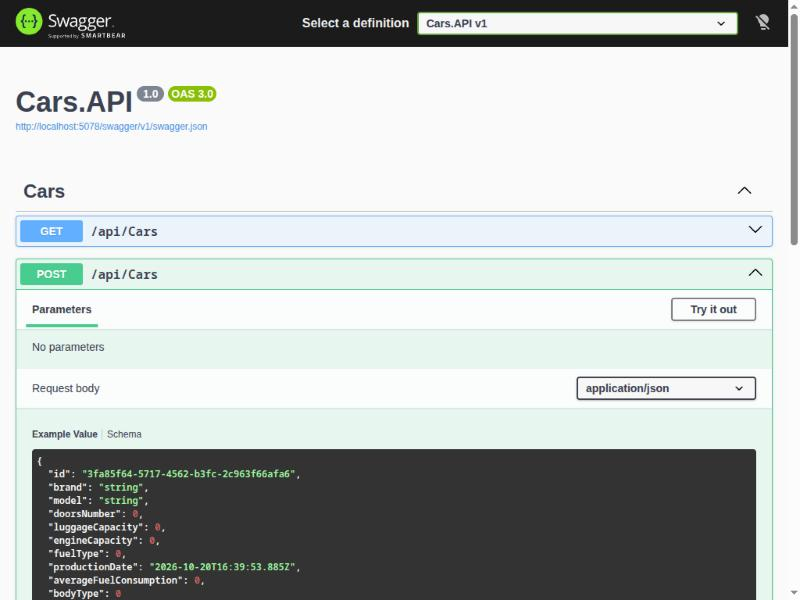
\includegraphics[width=0.66\textwidth]{img/swagger-post-schema.jpg}
    \caption{Swagger UI -- schemat treści żądania dla \texttt{POST /api/Cars} wygenerowany na podstawie modelu \texttt{Car}.}
\end{figure}

\clearpage
\subsection*{Zrzuty ekranu -- surowe odpowiedzi}

\Needspace{11cm}
\begin{figure}[H]
    \centering
    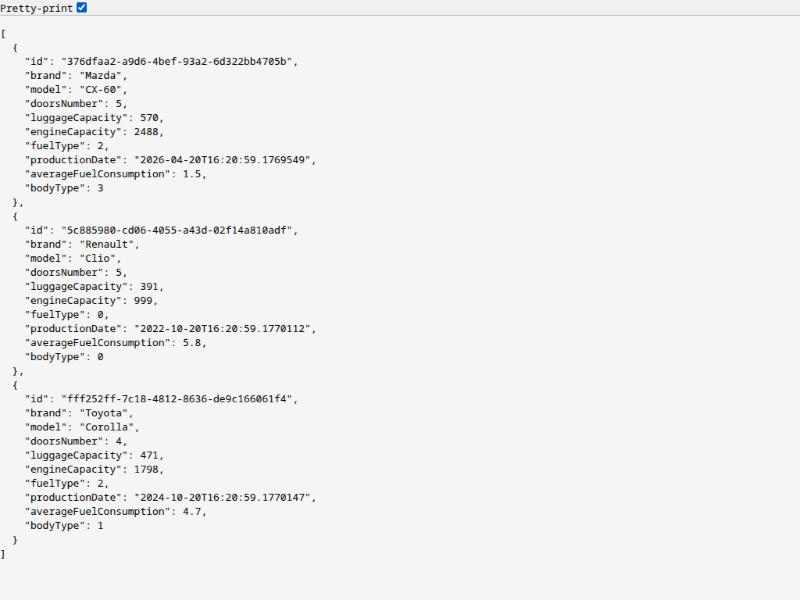
\includegraphics[width=0.66\textwidth]{img/get-cars.jpg}
    \caption{Odpowiedź \texttt{GET /api/cars} w przeglądarce (dane startowe wygenerowane przez \texttt{Seed.SeedData}).}
\end{figure}

\Needspace{11cm}
\begin{figure}[H]
    \centering
    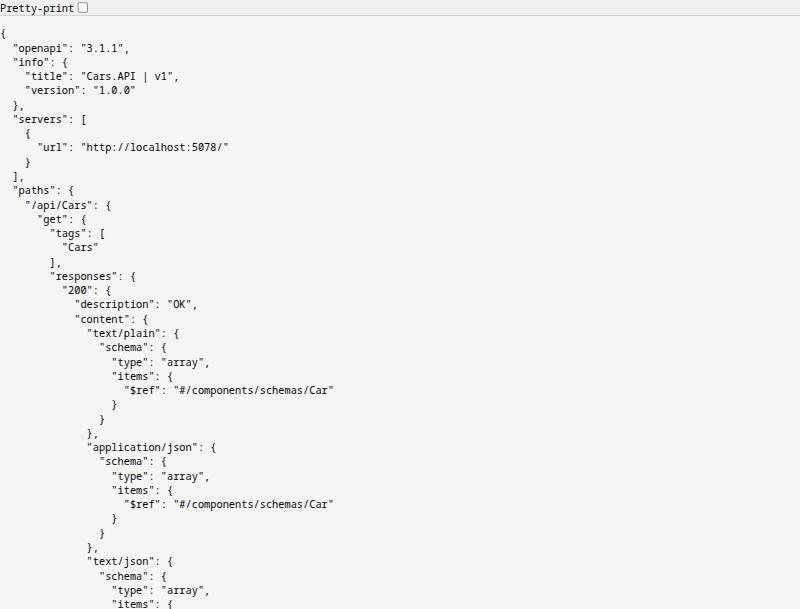
\includegraphics[width=0.66\textwidth]{img/openapi.jpg}
    \caption{Wygenerowany dokument OpenAPI (\texttt{/openapi/v1.json}) z zarejestrowanym endpointem \texttt{/api/Cars}.}
\end{figure}

\section*{\color{PSblue}3. Repozytorium GitHub}
{\small\color{PSgray}\textit{Podaj bezpośredni link do repozytorium zawierającego rozwiązanie zadania.}}

\begin{tabularx}{\textwidth}{>{\bfseries\color{PSblue}\columncolor{PSlight}}p{2.3cm} X}
Link: & \url{https://github.com/............................................................} \\
\end{tabularx}

\vfill
\begin{flushright}
{\small\color{PSgray}Data przygotowania: 20.10.2026}
\end{flushright}

\end{document}
